\chapter{Introducción}
\label{chap:introducción}
\section{Motivación}
Independientemente de la rama del desarrollo de los videojuegos en la que se pretenda trabajar, el factor decisivo que usan las empresas para determinar a qué profesional contratar son los juegos que ha desarrollado\cite{breaking_game_industry}. 

A través de la lista de juegos en las que una persona ha trabajado, los reclutadores y directores de recursos humanos pueden determinar la valía de un futuro empleado. Especialmente, sirve para valorar la capacidad de la persona para terminar un proyecto de gran envergadura, realizar una gestión de recursos correcta y su creatividad e iniciativa. De forma más específica, en el caso concrete do los programadores, una lista de proyectos completados (que pueden ser tanto juegos como herramientas de desarrollo) permite valorar su forma de desarrollar, mostrando si es capaz de escribir código comprensible y libre de errores.

La visibilidad que te da tener juegos completados no solo afecta a las empresas que buscan empleados. Tener una lista de juegos también sirve como carta de presentación para los jugadores, los cuales la podrán utilizar a la hora de decidir si deben o no adquirir un juego de dicho desarrollador, o invertir en una campaña de \textit{crownfunding}.

Desarrollar videojuegos también es beneficial para cualquier aspirante a desarrollador de videojuegos. Durante el desarrollo de cualquier videojuego se plantearán problemas (``¿Cómo se modela el comportamiento de un enemigo?'', ``¿Qué editor de niveles es más conveniente?'' ``¿Cuánto tiempo me llevará implementar esta característica concreta?'') los cuales muchas veces volverán a aparecer en muchos, sino todos, los futuros proyectos, por lo que con cada juego, el desarrollador ganará experiencia que le facilitará el trabajo en sus siguientes proyecto y le permitirá emprender proyectos cada vez más ambiciosos. 

Con estas ventajas en mente se eligió el desarrollo de un videojuego completo como proyecto de Fin de Grado.

\section{Diseño de juego}
\subsection{Concepto}
Este juego será de estilo-Breakout, género que se caracteriza por controlar una paleta con la que se redirige una pelota con el objetivo de destruir un muro de ladrillos o bloques. Sin embargo, este juego transcurrirá en un entorno totalmente tridimensional (a diferencia que otros juegos del género, los cuales tiene una área de juego bidimensional). 

En esta adaptación a las tres dimensiones, determinados elementos del juego han sido modificados respecto al estándar del género, inspirándose en otros juegos o deportes como el Squash \footnote{http://www.realfederaciondesquash.com/}

\begin{figure}[h]
	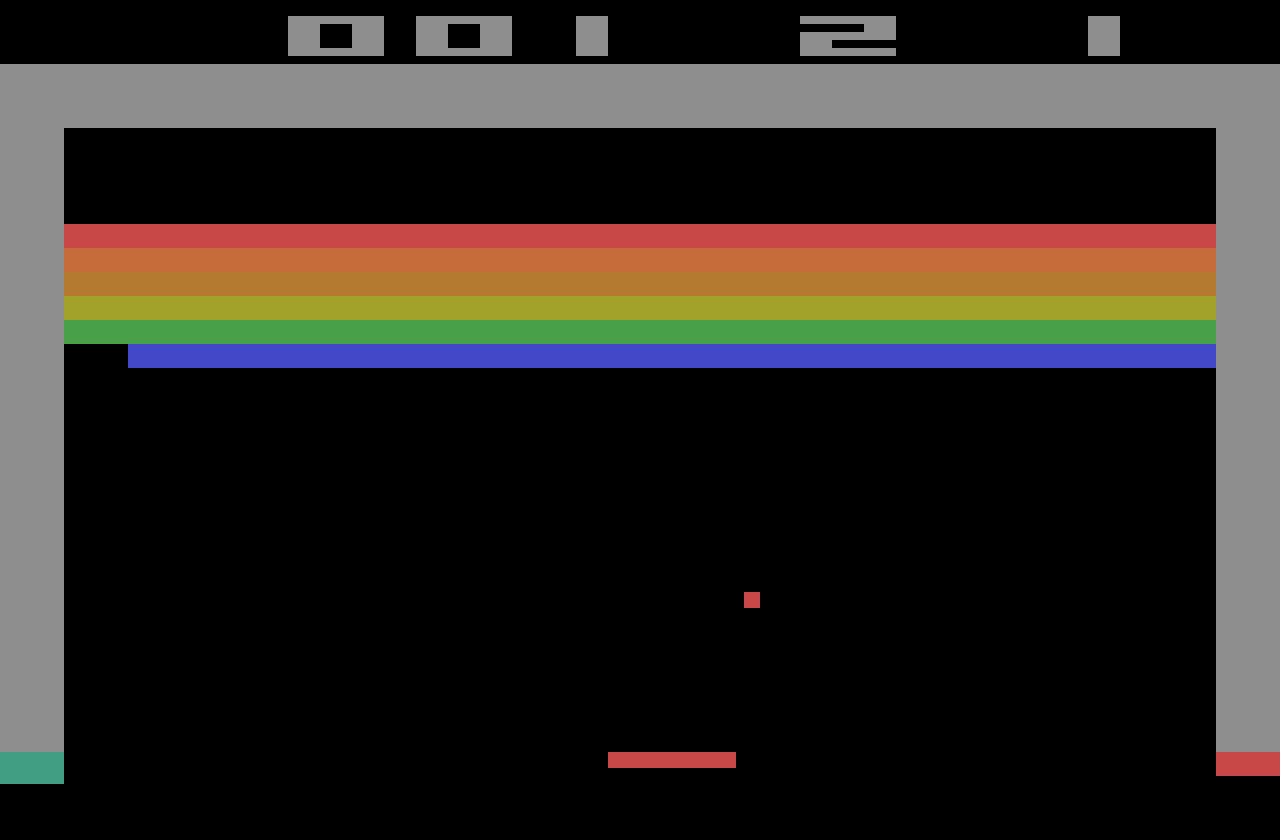
\includegraphics[width=0.8\textwidth]{images/intro/design/breakout}
	\centering
	\caption{Breakout (Atari, 1976)}
\end{figure}

\subsection{Jugabilidad}
En este juego, el jugador controla a un personaje encerrado en una sala cubica. El objetivo del juego es el de salir de la sala abriendo una enorme puerta que ocupa la totalidad de la pared norte de la sala. Para lograrlo, el jugador debe golpear una pelota usando una paleta para golpear con ella la puerta. Tras varios golpes, la puerta se abrirá. Sin embargo, la puerta estará cubierta por un muro de ladrillos que el jugador deberá romper primero para poder alcanzar la puerta. Por otro lado, si la pelota golpea tres veces consecutivas el suelo, el jugador perderá la partida.

El control del personaje principal es sencillo, ya que solo cuenta con dos acciones: moverse por el suelo de la sala y activar la paleta. El movimiento del personaje es un movimiento en ocho direcciones (delante, atrás, derecha, izquierda y diagonales), con una aceleración alta para dar una buena sensación de control. La activación de la paleta permitirá controlar la dirección de la bola, haciendo que esta rebote, impidiendo que caiga en al suelo y, idealmente, redirigiéndola hacia la puerta. La paleta estará activa durante un tiempo limitado, durante el cual el personaje permanecerá inmóvil. Si el personaje es golpeado por la pelota directamente, cuando la paleta está desactivada, el personaje quedará aturdido unos instantes, durante los cuales no podrá realizar ninguna acción.

La pelota se moverá por la sala rebotando de forma natural por sus paredes. Al golpear la puerta, o los bloques que la cubren, la pelota les causará daño. Los bloques se destruirán tras recibir daño suficiente, mientras que la puerta se abrirá, permitiendo al jugador salir de la sala. Si la pelota rebota tres veces en el suelo de la sala sin que el jugador la golpee con la paleta, esta será destruida y la partida se acabará.

La puerta de la sala está cubierta por un muro de ladrillos o bloques. Los bloques se colocan sobre la puerta alineados en una cuadricula de 16 X 16 unidades. Existen varios tipos de bloques, con distintas propiedades, los cuales pueden estar colocados con una rotación de 0º o de 90º y pintados de distintos colores. Los tipos de bloques son los siguientes:
\begin{itemize}
  \item Bloque Básico: Es el bloque normal, el cual se rompe al recibir un golpe de la pelota. Las dimensiones de este bloque son una unidad de altura y dos de anchura.
  \item Bloque Triple: Idéntico en dimensiones al bloque básico, pero se romperá tras recibir tres golpes en lugar de uno. 
  \item Bloque Divisible: Se trata de un bloque cuadrado de dos unidades de altura y anchura. Al ser golpeado, este bloque se romperá en cuatro Bloques Pequeños. 
  \item Bloque Pequeño: Es un bloque de pequeño tamaño (una unidad de altura y anchura).
  \item Bloque Irrompible: Este bloque no puede ser destruido por la pelota, por muchos golpes que reciba. Es también un bloque de gran tamaño, ya que mide el doble que el bloque básico (cuatro unidades de ancho y dos de altura).
\end{itemize}

El juego contendrá varias salas. Las salas tendrán unas dimensiones constantes, pero distintas configuraciones de bloques cubriendo la puerta, y distintos valores de ``puntos de vida'' para la puerta. Cuando el jugador abra la puerta de una sala, el personaje saldrá de ella y se moverá a otra sala distinta.  Las salas están ordenadas con dificultad creciente, de modo que el jugador se encontrará primero con las salas más sencillas antes de tener que enfrentarse a las más complicadas. Este aumento gradual mantendrá al jugador en un estado mental llamado ``fluir'' en el cual se tiene una concentración extrema en el juego \cite{flow}. De forma similar, los distintos tipos de bloques serán introducidos de forma progresiva.

\begin{figure}[h]
	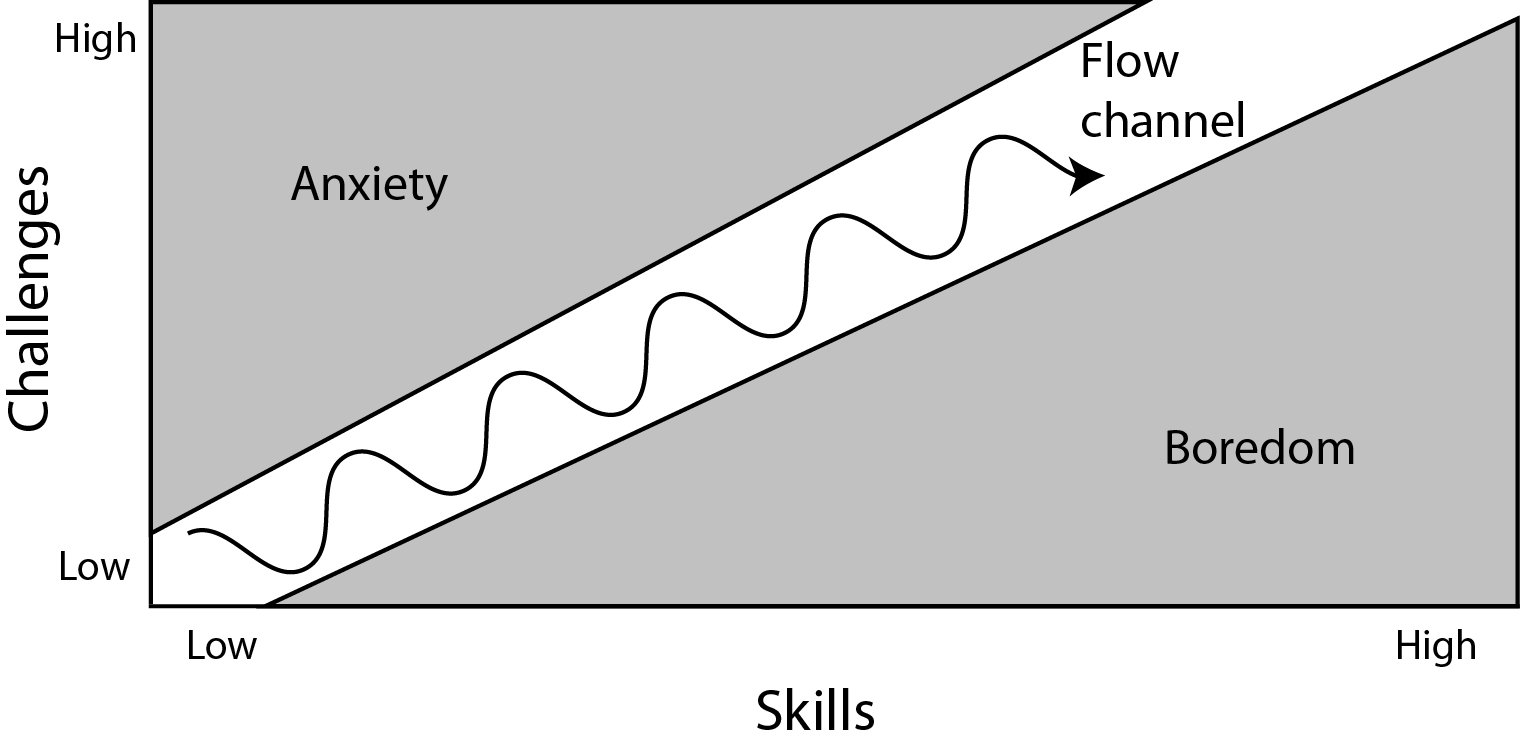
\includegraphics[width=0.8\textwidth]{images/intro/design/flow}
	\centering
	\caption{Relación entre desafío y la ansiedad/aburrimiento.}
\end{figure}

\subsection{Estilo y Ambientación}
El equipo de desarrollo de este juego está formado por una única persona, la cual debe realizar la producción completa del juego, que incluye diseño, programación, producción de los assets gráficos y creación de la música y sonidos. Dado que la responsabilidad de la producción artística cae en manos de un desarrollador que debe, además, ocuparse de otras responsabilidades dentro del proyecto en lugar de en un profesional que se dedique a tiempo completo en la producción, los posibles estilos gráficos y sonoros son limitados.

La elección del estilo artístico se limitaba a dos opciones: utilizar assets con licencia de libre uso, obtenidos de páginas como OpenGameArt.com\footnote{https://opengameart.org/}, o producir el arte utilizando un estilo sencillo y minimalista que pueda producirse en poco tiempo. La opción que se eligió fue la producción propia utilizando un estilo minimalista, ya que daría al juego un aspecto más único y cohesivo.
Dado que el diseño del juego requiere de gráficos tridimensionales, se optó por un diseño de personajes y escenarios con un bajo número de polígonos, al mismo tiempo que se empleaban texturas con una resolución y paleta de colores muy limitada, creadas usando el estilo artístico ``Pixel Art'', el cual imita las limitaciones gráficas de los ordenadores y videoconsolas antiguas. Los modelos resultantes de aplicar este estilo recuerdan a modelos de papel o maquetas construidas con bloques.

\begin{figure}[h]
	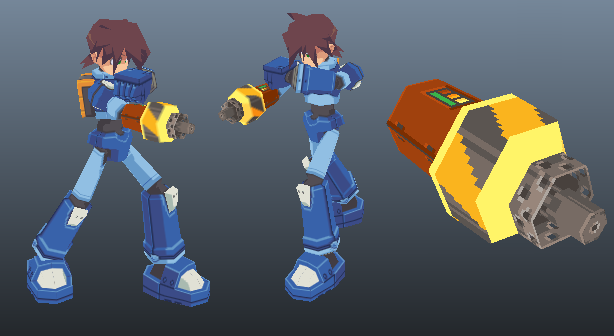
\includegraphics[width=0.8\textwidth]{images/intro/design/megaman}
	\centering
	\caption{El estilo del juego está influenciado por títulos como Megaman Legends(Capcom, 1997)}
\end{figure}

Las opciones para la producción musical son mucho más reducidas. Debido a la dificultad de crear una banda sonora desde cero, la única opción es utilizar música con licencia de libre uso. Para que la música esté en consonancia con el estilo artístico, se utilizará música de estilo ``Chiptune'' el cual, al igual que los gráficos, imita las limitaciones técnicas de videoconsolas y ordenadores antiguos. Esto mismo se aplicará a los efectos de sonido, también con licencia de libre uso e inspirados en los sonidos de videojuegos antiguos.

El estilo artístico resultante es muy ``Digital'', con polígonos visibles, pixeles de gran tamaño, colores limitados y música y sonido sintéticos. La consolidación de este estilo sirvió para definir la ambientación narrativa del juego: se decidió que el juego estará ambientado en el interior de un ordenador, con los personajes y entornos representando programas. Aunque el juego no hace uso de esta narrativa, al carecer de diálogos y cinemáticas, esta temática se empleó en el diseño de los gráficos.

\subsection{Plataforma}
Este juego ha sido diseñado para ser jugado en un PC. El control del personaje principal se realiza mediante las flechas de dirección (movimiento) y la tecla Espacio (paleta y navegar por menús). 

La exportación de este juego a dispositivos móviles como Android o IOS no sería posible debido a que el sistema de control no es compatible con pantallas táctiles, por lo que sería necesario realizar una adaptación, ya sea implementado un sistema de control del personaje basado en la pantalla táctil o mediante un controlador virtual en pantalla. Ambas aproximaciones aumentarían el coste de desarrollo del juego. Además, el juego no está optimizado para este tipo de dispositivos, de menor potencia que los PC, por lo que podría no funcionar correctamente.

La distribución del juego se realizará online, a través de las páginas de distribución de juegos Game Jolt\footnote{https://gamejolt.com/} y itch.io\footnote{https://itch.io/}. Estos sitios ofrecen a sus usuarios la posibilidad de subir, sin ningún tipo de coste, el juego a la página para que otros usuarios puedan descargarlos (o, en el caso de Game Jolt, jugarlos directamente en el navegador si el juego es compatible). Ambas páginas ofrecen la posibilidad tanto de vender el juego como de distribuirlo de forma gratuita. Dada la naturaleza del proyecto, se ha optado por la distribución gratuita del mismo.
\begin{figure}[!htb]
   \begin{minipage}{0.50\textwidth}
     \centering
     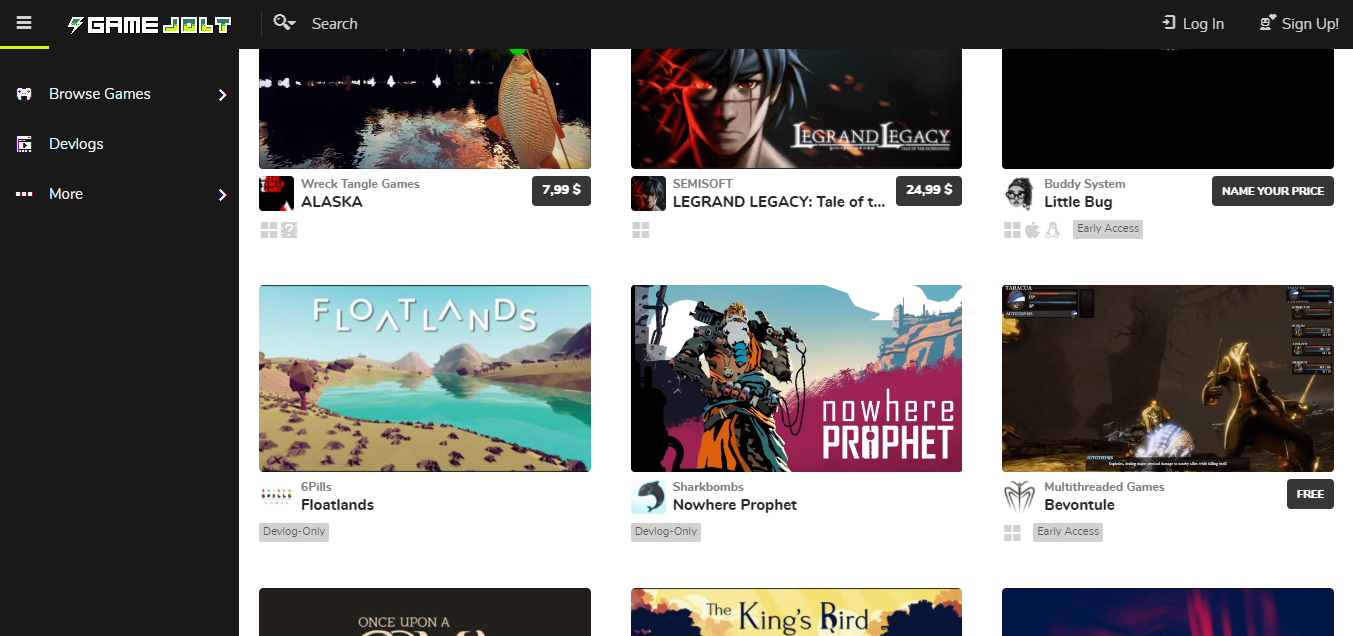
\includegraphics[width=0.9\linewidth, left]{images/intro/design/gamejolt}
     \caption{Gamejolt}
   \end{minipage}\hfill
   \begin {minipage}{0.50\textwidth}
     \centering
     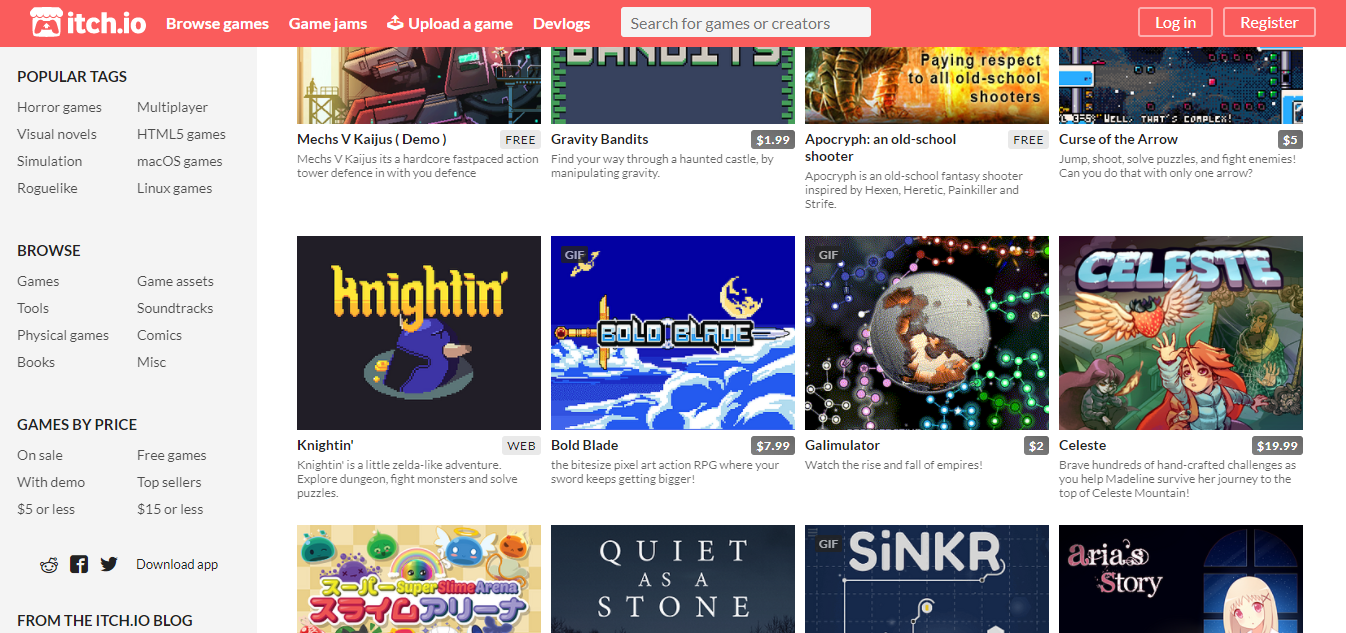
\includegraphics[width=0.9\linewidth, right]{images/intro/design/itchio}
     \caption{Itch.io}
   \end{minipage}
   \caption{Juegos desarrollados con Unity3D}
\end{figure}
